\documentclass[../linear-algebra.tex]{subfiles}
\begin{document}

\section{Vectors}
\subsection{2-D, 3-D}

Scalar: Only magnitude, notation: $a, t, x, y$

\noindent Vector: Magnitude \& direction, notation: \textbf{f, x, v, w}

\noindent Vectors \textbf{v} = \textbf{w} if they have the same length \& direction.\newline
Origin point does not matter.

\begin{center} 
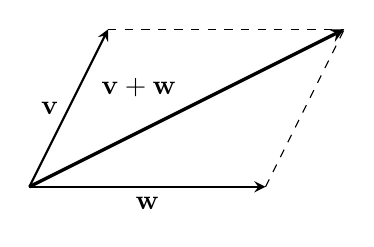
\begin{tikzpicture}[>=stealth, thick]
    \coordinate (O) at (0,0);
    \coordinate (V) at (1,2);
    \coordinate (W) at (3,0);
    \coordinate (VW) at (4,2); 

    \draw[->] (O) -- (V) node[midway, left] {$\mathbf{v}$};
    \draw[->] (O) -- (W) node[midway, below] {$\mathbf{w}$};
    \draw[->, very thick] (O) -- (VW) node[midway, above left] {$\mathbf{v+w}$};

    \draw[dashed, thin] (V) -- (VW);
    \draw[dashed, thin] (W) -- (VW);
\end{tikzpicture}
\hfil 
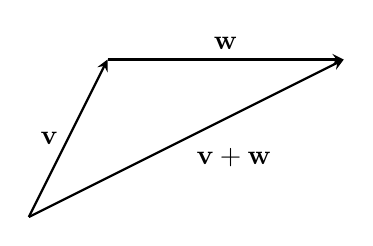
\begin{tikzpicture}[>=stealth, thick]
    \coordinate (O) at (0,0);
    \coordinate (V) at (1,2);
    \coordinate (VW) at (4,2); 

    \draw[->] (O) -- (V) node[midway, left] {$\mathbf{v}$};
    \draw[->] (V) -- (VW) node[midway, above] {$\mathbf{w}$};
    \draw[->] (O) -- (VW) node[midway, below right] {$\mathbf{v+w}$};
\end{tikzpicture}
\end{center}

\noindent Vector addition: Parallelogram rule and Triangle rule give the same result.

\begin{center}
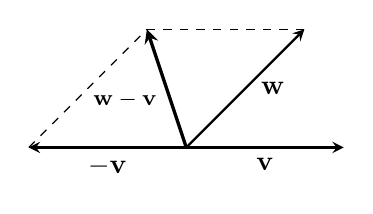
\begin{tikzpicture}[>=stealth, thick]
    \coordinate (O) at (0,0);
    \coordinate (V) at (2,0);
    \coordinate (W) at (1.5,1.5);
    \coordinate (negV) at (-2,0);
    \coordinate (diff) at (-0.5,1.5); 

    \draw[->] (O) -- (V) node[midway, below] {$\mathbf{v}$};
    \draw[->] (O) -- (negV) node[midway, below] {$\mathbf{-v}$};
    
    \draw[->] (O) -- (W) node[midway, right, right=2pt] {$\mathbf{w}$};
    
    \draw[->, very thick] (O) -- (diff) node[pos=0.4, left=1pt] {\footnotesize $\mathbf{w-v}$};

    \draw[dashed, thin] (W) -- (diff);
    \draw[dashed, thin] (negV) -- (diff);
\end{tikzpicture}
\hfil 
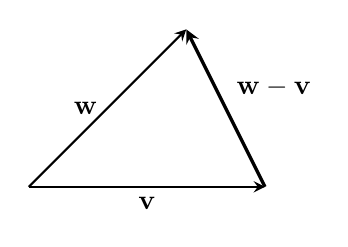
\begin{tikzpicture}[>=stealth, thick]
    \coordinate (O) at (0,0);
    \coordinate (V) at (3,0);
    \coordinate (W) at (2,2);

    \draw[->] (O) -- (V) node[midway, below] {$\mathbf{v}$};
    \draw[->] (O) -- (W) node[midway, left] {$\mathbf{w}$};

    \draw[->, very thick] (V) -- (W) node[midway, above right] {$\mathbf{w-v}$};
\end{tikzpicture}
\end{center}

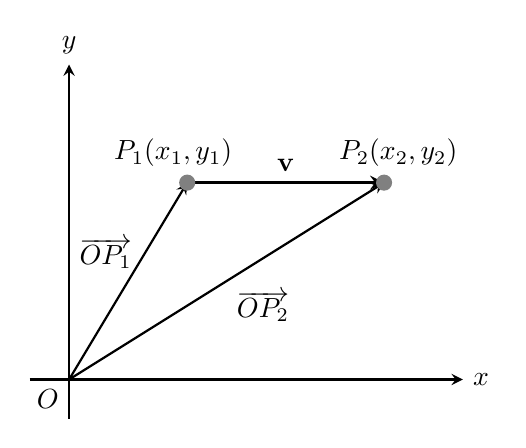
\begin{tikzpicture}[>=stealth, thick]
    % Draw Axes and Origin
    \draw[->] (-0.5,0) -- (5,0) node[right] {$x$};
    \draw[->] (0,-0.5) -- (0,4) node[above] {$y$};
    \node[below left] at (0,0) {$O$};

    % Define Coordinates
    \coordinate (O) at (0,0);
    \coordinate (P1) at (1.5,2.5);
    \coordinate (P2) at (4,2.5);

    % Draw Position Vectors from Origin
    % yshift=5pt moves the label higher up along the line
    \draw[->] (O) -- (P1) node[midway, left, yshift=10pt, xshift=5pt] {$\overrightarrow{OP_1}$};
    \draw[->] (O) -- (P2) node[midway, below right] {$\overrightarrow{OP_2}$};

    % Draw Displacement Vector v
    \draw[->, very thick] (P1) -- (P2) node[midway, above] {$\mathbf{v}$};

    \filldraw[gray] (P1) circle (2.5pt) node[above left, xshift=20pt, yshift=2pt, black] {$P_1(x_1, y_1)$};
    \filldraw[gray] (P2) circle (2.5pt) node[above right, xshift=-20pt, yshift=2pt, black] {$P_2(x_2, y_2)$};
\end{tikzpicture}

\noindent Vector subtraction.
$\mathbf{v} = \overrightarrow{P_1P_2} = \overrightarrow{P_1O} + \overrightarrow{OP_2} =
\overrightarrow{OP_2} - \overrightarrow{OP_1}$

\begin{center}
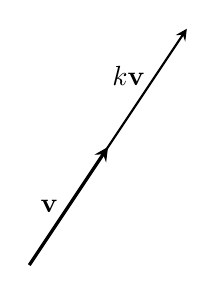
\begin{tikzpicture}[>=stealth, thick]
    \coordinate (O) at (0,0);
    \coordinate (V) at (1,1.5);
    \coordinate (KV) at (2,3);

    \draw[->] (O) -- (KV) node[pos=0.8, left] {$k\mathbf{v}$};
    \draw[->, very thick] (O) -- (V) node[midway, left] {$\mathbf{v}$};
\end{tikzpicture}
\hfil
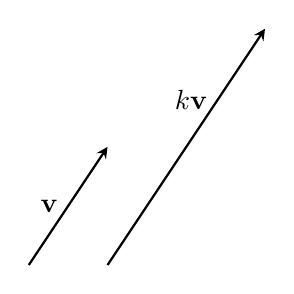
\begin{tikzpicture}[>=stealth, thick]
    \coordinate (O1) at (0,0);
    \coordinate (V) at (1,1.5);
    
    \coordinate (O2) at (1,0);
    \coordinate (KV) at (3,3);

    \draw[->] (O1) -- (V) node[midway, left] {$\mathbf{v}$};
    
    \draw[->] (O2) -- (KV) node[pos=0.7, left] {$k\mathbf{v}$};
\end{tikzpicture}
\end{center}

\noindent Scalar multiple $k$\textbf{v} of the vector \textbf{v} is the same
whether it is collinear or parallel.

\begin{center}
    \begin{minipage}[t]{0.45\textwidth}
        \centering
        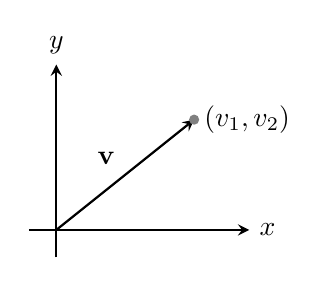
\begin{tikzpicture}[>=stealth, thick, scale=0.7]
            \draw[->] (-0.5,0) -- (3.5,0) node[right] {$x$};
            \draw[->] (0,-0.5) -- (0,3) node[above] {$y$};
            \coordinate (V) at (2.5,2);
            \draw[->] (0,0) -- (V) node[midway, above left] {$\mathbf{v}$};
            \filldraw[gray] (V) circle (2pt) node[right, black] {$(v_1, v_2)$};
        \end{tikzpicture}
        
        \vspace{0.5cm}
        $\mathbf{v} = (v_1, v_2)$ or $\begin{bmatrix} v_1 \\ v_2 \end{bmatrix}$
    \end{minipage}
    \hfill
    \begin{minipage}[t]{0.45\textwidth}
        \centering
        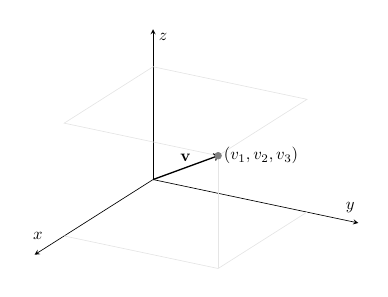
\begin{tikzpicture}[scale=0.6]
        \begin{axis}[
            view={120}{30}, axis lines=center,
            xlabel=$x$, ylabel=$y$, zlabel=$z$,
            xmin=0, xmax=4, ymin=0, ymax=4, zmin=0, zmax=4,
            ticks=none, axis line style={->, >=stealth}, clip=false
        ]
            \coordinate (V) at (axis cs:3,3,3);
            \draw[gray!20] (axis cs:3,0,0) -- (axis cs:3,3,0) -- (axis cs:0,3,0);
            \draw[gray!20] (axis cs:3,3,0) -- (axis cs:3,3,3);
            \draw[gray!20] (axis cs:0,0,3) -- (axis cs:3,0,3) -- (axis cs:3,3,3) -- (axis cs:0,3,3) -- cycle;
            \draw[->, thick] (axis cs:0,0,0) -- (V) node[midway, above] {$\mathbf{v}$};
            \filldraw[gray] (V) circle (2pt) node[right, black] {$(v_1, v_2, v_3)$};
        \end{axis}
        \end{tikzpicture}
        
        \vspace{0.5cm}
        $\mathbf{v} = (v_1, v_2, v_3)$
    \end{minipage}
\end{center}
Two vectors $\mathbf{v}$ = $(v_1, v_2, v_3)$, $\mathbf{w}$ = $(w_1, w_2, w_3)$
are equal iff $v_1 = w_1, v_2 = w_2, v_3 = w_3$.

\bigskip

\subsection{\textit{n}-D space}

\noindent Real line: $\mathbb{R}^1$

\noindent $\mathbf{v} \in \mathbb{R}^2: \mathbf{v} = (v_1, v_2)$

\noindent $\mathbf{v} \in \mathbb{R}^3: \mathbf{v} = (v_1, v_2, v_3)$

\noindent $\mathbf{v} \in \mathbb{R}^n: \mathbf{v} = (v_1, v_2, \ldots, v_n)$
(Set of all ordered \textit{n}-tuples called \textit{n}-D space).

\noindent Zero vector $\mathbf{v} \in \mathbb{R}^n: \mathbf{v} = \mathbf{0} = (0, 0, \ldots, 0)$ 

\paragraph{Definition}
If $\mathbf{v} = (v_1, v_2, \ldots, v_n)$ and $\mathbf{w} = (w_1, w_2, \ldots, w_n)$
in $\mathbb{R}^n$, and for any scalar $k$, then
\begin{enumerate}
    \item $\mathbf{v} + \mathbf{w} = (v_1 + w_1, v_2 + w_2, \ldots, v_n + w_n)$
    \item $k\mathbf{v} = (kv_1, kv_2, \ldots, kv_n)$
    \item $-\mathbf{v} = (-v_1, -v_2, \ldots, -v_n)$
    \item $\mathbf{w} - \mathbf{v} = \mathbf{w} + (-\mathbf{v})
    = (w_1 - v_1, w_2 - v_2, \ldots, w_n - v_n)$
\end{enumerate}

\paragraph{Theorem}
If $\mathbf{u}, \mathbf{v}$ and $\mathbf{w}$ are vectors in $\mathbb{R}^n$,
and if $k$ and $m$ are scalars, then
\begin{enumerate}
    \item $\mathbf{u} + \mathbf{v} = \mathbf{v} + \mathbf{u}$
    \item $(\mathbf{u} + \mathbf{v}) + \mathbf{w} = \mathbf{u} + (\mathbf{v} + \mathbf{w})$
    \item $\mathbf{u} + 0 = 0 + \mathbf{u} = \mathbf{u}$
    \item $\mathbf{u} + (-\mathbf{u}) = 0$
    \item $k(\mathbf{u} + \mathbf{v}) = k\mathbf{u} + k\mathbf{v}$
    \item $(k + m)\mathbf{u} = k\mathbf{u} + m\mathbf{u}$
    \item $k(m\mathbf{u}) = (km)\mathbf{u}$
    \item $1\mathbf{u} = \mathbf{u}$
    \item $0\mathbf{v} = 0$
    \item $k0 = 0$
    \item $-1\mathbf{v} = -\mathbf{v}$
\end{enumerate}

\paragraph{Linear combination}
If $\mathbf{w}$ is a vector in $\mathbb{R}^n$, then $\mathbf{w}$ is a linear
combination of vectors $v_1, v_2,\ldots, v_n$ in $\mathbb{R}^n$ if it can be
expressed in the from
\[\mathbf{w} = k_1\mathbf{v_1} + k_2\mathbf{v_2} +\ldots + k_n\mathbf{v_n}\]
where $k_1, k_2, \ldots, k_n$ are scalars and the coefficients of the linear combination.

\subsection{Norm, Dot Product and Distance in $\mathbb{R}^n$}

\begin{center}
    \begin{minipage}{0.7\textwidth}
        \centering
        
        \begin{minipage}{0.5\textwidth}
            \centering
            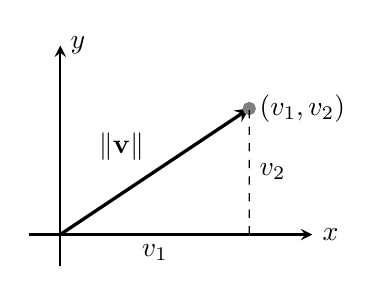
\begin{tikzpicture}[>=stealth, thick, scale=0.8]
                \draw[->] (-0.5,0) -- (4,0) node[right] {$x$};
                \draw[->] (0,-0.5) -- (0,3) node[right] {$y$};
                
                \coordinate (V) at (3,2);
                \draw[->, very thick] (0,0) -- (V) node[midway, above left] {$\|\mathbf{v}\|$};
                \filldraw[gray] (V) circle (2.5pt) node[right, black] {$(v_1, v_2)$};
                
                \draw[dashed, thin] (3,0) -- (V);
                \node[below] at (1.5,0) {$v_1$};
                \node[right] at (3,1) {$v_2$};
            \end{tikzpicture}
        \end{minipage}
        \hfill
        \begin{minipage}{0.4\textwidth}
            \centering
            \[
            \|\mathbf{v}\| = \sqrt{v_1^2 + v_2^2}
            \]
        \end{minipage}
    \end{minipage}
\end{center}

\noindent For a vector $\mathbf{v} = (v_1, v_2,\ldots, v_n)$ in $\mathbb{R}^n$,
the norm/length/magnitude of $\mathbf{v}$ is
\[\|\mathbf{v}\| = \sqrt{v_1^2 + v_2^2 + \dots + v_n^2}\]

\paragraph{Norm of a vector}
For vectors $\mathbf{v}$, $\mathbf{w}$ in $\mathbb{R}^n$ and a scalar $k$,
\begin{enumerate}
    \item $\|\mathbf{v}\| \geq 0$
    \item $\|\mathbf{v}\| = 0 \iff \mathbf{v} = 0$
    \item $\|k\mathbf{v}\| = |k|\|\mathbf{v}\|$
    \item $\|\mathbf{v} + \mathbf{w}\| \leq \|\mathbf{v}\| + \|\mathbf{w}\|$
\end{enumerate}

\paragraph{Unit vector}
For $\mathbf{v}$ a nonzero vector in $\mathbb{R}^n$, by normalising $\mathbf{v}$
we get a unit vector $\mathbf{u}$, with the same direction as $\mathbf{v}$,
defined as
\[\mathbf{u} = \frac{1}{\|\mathbf{v}\|}\mathbf{v}\]

\noindent Standard unit vectors are unit vectors that point along the positive axes
of the coordinate axes.

\noindent In $\mathbb{R}^3$, standard unit vectors are $\mathbf{i} = (1, 0, 0)$, $\mathbf{j} = (0, 1, 0)$, $\mathbf{k} = (0, 0, 1)$.

\noindent In $\mathbb{R}^n$, we have standard unit vectors

$\mathbf{e}_1 = (1, 0, 0, \ldots, 0), \mathbf{e}_2 = (0, 1, 0, \ldots, 0), \mathbf{e}_3 = (0, 0, \ldots, 1)$.

\paragraph{Distance in $\mathbb{R}^n$}
For points $\mathbf{u} = (u_1, u_2, \ldots, u_n)$, $\mathbf{v} = (v_1, v_2, \ldots, v_n)$ in $\mathbb{R}^n$,
the distance between $\mathbf{u}$ and $\mathbf{v}$ is
\[d(\mathbf{u}, \mathbf{v}) = \|\mathbf{u} - \mathbf{v}\|
= \sqrt{(u_1 - v_1)^2 + (u_2 - v_2)^2 + \ldots + (u_n - v_n)^2}\]

\subsubsection*{Dot Product}

For two vectors $\mathbf{u}$ and $\mathbf{v}$ in $\mathbb{R}^n$, their dot product (in geometric form) is
\[\mathbf{u} \cdot \mathbf{v} = \|\mathbf{u}\|\|\mathbf{v}\|\cos\theta\]

\noindent The component form of the dot product is
\[\mathbf{u} \cdot \mathbf{v} = u_1v_1 + u_2v_2 + \ldots + u_nv_n\]

\noindent Since $\cos\theta = \frac{\mathbf{u} \cdot \mathbf{v}}{\|u\|\|v\|}$,
\begin{itemize}
    \item If $\mathbf{u} \cdot \mathbf{v} > 0$, $0 \leq \theta < \frac{\pi}{2}$
    \item If $\mathbf{u} \cdot \mathbf{v} < 0$, $\frac{\pi}{2} < \theta \leq \pi$
    \item If $\mathbf{u} \cdot \mathbf{v} = 0$, $\theta = \frac{\pi}{2}$
\end{itemize}

\subsubsection{Properties}

$\mathbf{v} \cdot \mathbf{v} = v_1^2 + v_2^2 + \ldots + v_n^2 = \|v\|^2$

\medskip

\noindent We can get length of a vector in terms of its dot product: $\|v\| = \sqrt{\mathbf{v}\cdot\mathbf{v}}$

\medskip

\noindent For vectors $\mathbf{u}$, $\mathbf{v}$, $\mathbf{w}$ in $\mathbb{R}^n$ and $k$ a scalar,
\begin{enumerate}
    \item $\mathbf{u} \cdot \mathbf{v} = \mathbf{v} \cdot \mathbf{u}$ [Symmetry]
    \item $\mathbf{u}(\mathbf{v} + \mathbf{w}) = \mathbf{u} \cdot \mathbf{v} + \mathbf{u} \cdot \mathbf{w}$ [Distributivity]
    \item $k(\mathbf{u} \cdot \mathbf{v}) = (k\mathbf{u})\cdot\mathbf{v}$ [Homogeneity]
    \item $\mathbf{v}\cdot\mathbf{v} \geq 0$ and $\mathbf{v}\cdot\mathbf{v} = 0 \iff \mathbf{v} = \mathbf{0}$ [Positivity]
    \item $\mathbf{0}\cdot\mathbf{v} = \mathbf{v}\cdot\mathbf{0} = 0$
    \item $(\mathbf{u} + \mathbf{v})\cdot\mathbf{w} = \mathbf{u}\cdot\mathbf{w} + \mathbf{v}\cdot\mathbf{w}$
    \item $\mathbf{u}\cdot(\mathbf{v} - \mathbf{w}) = \mathbf{u}\cdot\mathbf{v} - \mathbf{u}\cdot\mathbf{w}$
    \item $(\mathbf{u} - \mathbf{v}) \cdot \mathbf{w} = \mathbf{u} \cdot \mathbf{w} - \mathbf{v} \cdot \mathbf{w}$
    \item $k(\mathbf{u} \cdot \mathbf{v}) = \mathbf{u} \cdot (k\mathbf{v})$
\end{enumerate}

\paragraph{Cauchy-Schwarz Inequality}
If $\mathbf{u} = (u_1, u_2, \ldots, u_n)$ and $\mathbf{v} = (v_1, v_2, \ldots, v_n)$
are vectors in $\mathbb{R}^n$, then
\[|\mathbf{u}\cdot\mathbf{v}| \leq \|\mathbf{u}\|\|\mathbf{v}\|\]
Hence, $-1 \leq \frac{\mathbf{u}\cdot\mathbf{v}}{\|\mathbf{u}\|\mathbf{v}\|} \leq 1$,
and $\theta$ is always defined,
where $\theta = \arccos(\frac{\mathbf{u}\cdot\mathbf{v}}{\|\mathbf{u}\|\mathbf{v}\|})$.

\paragraph{Triangle Inequality}
For vectors $\mathbf{u}$, $\mathbf{v}$ and $\mathbf{w}$ in $\mathbb{R}^n$ and a scalar $k$,
\begin{enumerate}
    \item $\|\mathbf{u} + \mathbf{v}\| \leq \|\mathbf{u}\| + \|\mathbf{v}\|$ [For vectors]
    \item $d(\mathbf{u}, \mathbf{v}) \leq d(\mathbf{u}, \mathbf{w}) + d(\mathbf{w}, \mathbf{v})$ [For distances]
\end{enumerate}

\paragraph{Orthogonality}
Two nonzero vectors $\mathbf{u}$ and $\mathbf{v}$ in $\mathbb{R}^n$
are orthogonal if $\mathbf{u}\cdot\mathbf{v} = 0$.
This means the two vectors are perpendicular to each other, from
\[\theta = \cos^{-1}\left(\frac{\mathbf{u}\cdot\mathbf{v}}{\|u\|\|v\|}\right)\]
A nonempty set of vectors in $\mathbb{R}^n$ is an orthogonal set if all
pairs of distinct vectors in the set are orthogonal.

\subsubsection*{Equations of lines and planes}

\noindent % Prevents indentation of the first minipage
\begin{minipage}{0.48\textwidth}
    \centering
    \begin{tikzpicture}[>=Stealth, thick, scale=0.8] % Scale slightly to fit well
        % Draw Axes
        \draw[->] (-1,0) -- (5,0) node[right] {$x$};
        \draw[->] (0,-1) -- (0,4) node[above] {$y$};

        % Define points for the line
        \coordinate (P0) at (2,1);
        \coordinate (P) at (0.5,2.5);
        
        % Draw the infinite line
        \draw[shorten <=-2cm, shorten >=-2cm, thin, gray!60] (P0) -- (P);

        % Draw the normal vector n
        \coordinate (N) at (3.5, 2.5); 
        \draw[->, ultra thick] (P0) -- (N) node[midway, right, xshift=2pt] {$\mathbf{n} = (a, b)$};

        % Draw the vector from P0 to P
        \draw[->, thick] (P0) -- (P);
        
        % Add Labels for points
        \filldraw (P0) circle (2pt) node[below] {$P_0(x_0, y_0)$};
        \filldraw (P) circle (2pt) node[above right] {$P(x, y)$};

        % Draw the Right Angle Symbol
        \draw[thin] (2.2, 1.2) -- (2.0, 1.4) -- (1.8, 1.2);
    \end{tikzpicture}
\end{minipage}
\hfill % Adds horizontal space to push diagrams to the edges
\begin{minipage}{0.48\textwidth}
    \centering
    \tdplotsetmaincoords{70}{110}
    \begin{tikzpicture}[tdplot_main_coords, >=Stealth, thick, scale=0.8]
        % 1. Draw Coordinate Axes
        \draw[->] (0,0,0) -- (4,0,0) node[anchor=north east]{$x$};
        \draw[->] (0,0,0) -- (0,5,0) node[anchor=north west]{$y$};
        \draw[->] (0,0,0) -- (0,0,4) node[anchor=south]{$z$};

        % 2. Define Points for the Plane
        \coordinate (A) at (3,0,0);
        \coordinate (B) at (0,4,0);
        \coordinate (C) at (0,0,3);
        
        \fill[gray, opacity=0.3] (A) -- (B) -- (C) -- cycle;
        \draw[thin, black!60] (A) -- (B) -- (C) -- cycle;

        % 3. Define P0 and P
        \coordinate (P0) at (1, 1, 1.25); 
        \coordinate (P)  at (0.5, 2.5, 0.75); 
        
        % 4. Draw vector P0P
        \draw[->, ultra thick] (P0) -- (P);
        
        % 5. Draw Normal Vector 'n'
        \coordinate (N_end) at (2.5, 2.5, 3.5);
        \draw[->, ultra thick] (P0) -- (N_end) node[midway, right] {$\mathbf{n}$};
        \filldraw (N_end) circle (3pt) node[above right] {$(a, b, c)$};

        % 6. Add Labels
        \filldraw (P0) circle (2pt) node[below left] {$P_0(x_0, y_0, z_0)$};
        \filldraw (P) circle (2pt) node[above] {$P(x, y, z)$};

        % 7. Draw the Orthogonality Symbol
        \draw[thin] (1.1, 1.2, 1.4) -- (1.3, 1.4, 1.6) -- (1.2, 1.3, 1.45);
    \end{tikzpicture}
\end{minipage}

\noindent For \textbf{point-normal equations}, we need two things:
\begin{enumerate}
    \item Coordinates of a point on the line/plane, $P_0$.
    \item The normal from that point, $\mathbf{n}$, which is orthogonal to the line/plane.
\end{enumerate}

\noindent We make use of the property $\mathbf{n}\cdot\overrightarrow{P_0P} = 0$,
where $P$ is the variable point of the line/plane.

\bigskip

\noindent For a line (in $\mathbb{R}^n$):
\begin{align*}
\mathbf{n} \cdot \overrightarrow{P_0P} &= 0 \\
\overrightarrow{P_0P} &= (x - x_0, y - y_0) \\
\mathbf{n} &= (a, b) \\
a(x - x_0) + b(y - y_0) &= 0
\end{align*}

\noindent For a plane:
\begin{align*}
\mathbf{n} \cdot \overrightarrow{P_0P} &= 0 \\
\overrightarrow{P_0P} &= (x - x_0, y - y_0, z - z_0) \\
\mathbf{n} &= (a, b, c) \\
a(x - x_0) + b(y - y_0) + c(z - z_0) &= 0
\end{align*}

\noindent If $ax + by + cz = 0$, then the line/plane passes through the origin.\newline
Note that the coefficients of the line/plane are the normal vector values.


\subsubsection*{Vector/Parametric Equations}

\noindent
%% --- Left Diagram: Parametric Line ---
\begin{minipage}{0.48\textwidth}
\centering
\begin{tikzpicture}[>=Stealth, thick, scale=0.8]
    % Draw Axes
    \draw[->] (-0.5,0) -- (4.5,0) node[right] {$x$};
    \draw[->] (0,-0.5) -- (0,4) node[above] {$y$};

    % Define points with matching slopes for parallelism
    % Slope is 0.5 (1 unit up for every 2 units right)
    \coordinate (X0) at (1,1.5);
    \coordinate (X) at (3,2.5);
    \coordinate (V) at (2,1); % Direction vector v from origin

    % Draw the infinite line L
    \draw[gray!40, thin, shorten <=-1cm, shorten >=-1cm] (X0) -- (X) node[black, right, xshift=5pt] {$L$};

    % Draw vector x - x0
    \draw[->, very thick] (X0) -- (X) node[midway, above left, yshift=2pt] {$\mathbf{x} - \mathbf{x}_0$};

    % Draw points
    \filldraw[gray] (X0) circle (3.5pt) node[black, above left] {$\mathbf{x}_0$};
    \filldraw[gray] (X) circle (3.5pt) node[black, above, yshift=4pt] {$\mathbf{x}$};

    % Draw direction vector v from origin (perfectly parallel to L)
    \draw[->, very thick] (0,0) -- (V) node[midway, above left] {$\mathbf{v}$};
\end{tikzpicture}
\end{minipage}
\hfill
%% --- Right Diagram: Parametric Plane ---
\begin{minipage}{0.48\textwidth}
\centering
\tdplotsetmaincoords{70}{120}
\begin{tikzpicture}[tdplot_main_coords, >=Stealth, thick, scale=0.8]
    % Draw Coordinate Axes
    \draw[->] (0,0,0) -- (4,0,0) node[anchor=north east]{$x$};
    \draw[->] (0,0,0) -- (0,5,0) node[anchor=north west]{$y$};
    \draw[->] (0,0,0) -- (0,0,4) node[anchor=south]{$z$};

    % Define Plane corners (floating sheet)
    \coordinate (C1) at (0, 1, 3);
    \coordinate (C2) at (3, 0, 1);
    \coordinate (C3) at (5, 4, 1);
    \coordinate (C4) at (2, 5, 3);

    % Shaded Plane W
    \fill[gray!20, opacity=0.6] (C1) -- (C2) -- (C3) -- (C4) -- cycle;
    \draw[thin, black!60] (C1) -- (C2) -- (C3) -- (C4) -- cycle;
    \node at (C4) [above right] {$W$};

    % Define Points and Vectors on the plane
    \coordinate (X0) at (0, 0, 0);
    \coordinate (X) at (2, 3, 3);
    \coordinate (V1_end) at (3, 4, 3); 
    \coordinate (V2_end) at (4, 3, 4);

    % Draw spanning vectors t1v1 and t2v2
    \draw[->, very thick] (X0) -- (V1_end) node[midway, below, xshift=5pt] {$t_1\mathbf{v}_1$};
    \draw[->, very thick] (X0) -- (V2_end) node[midway, left] {$t_2\mathbf{v}_2$};
    
    % Draw projection lines to point x
    \draw[dashed, gray!80, thin] (V1_end) -- (X);
    \draw[dashed, gray!80, thin] (V2_end) -- (X);

    % Draw resultant vector from X0 to X
    \draw[->, thick] (X0) -- (X) node[midway, above right] {};

    % Label points
    \filldraw[gray] (X0) circle (3pt) node[black, left] {$\mathbf{x}_0$};
    \filldraw[gray] (X) circle (3pt) node[black, above right, yshift=-4pt, xshift=2pt] {$\mathbf{x}$};
\end{tikzpicture}
\end{minipage}

\bigskip

\noindent For a line containing point $x_0$ and parallel to vector $\mathbf{v}$,
the vector form is
\[\mathbf{x} - \mathbf{x_0} = t\mathbf{v}\]
and the parametric form is
\begin{align*}
    x &= x_0 + ta \\
    y &= y_0 + tb \\
    z &= z_0 + tc
\end{align*}

\noindent For a vector containing point $x_0$ and parallel to noncollinear vectors $v_1$ and $v_2$,
the vector form is 
\[\mathbf{x} - \mathbf{x}_0 = t_1\mathbf{v}_1 + t_2\mathbf{v}_2\]
and the parametric form is
\begin{align*}
    x &= x_0 + t_1a_1 + t_2a_2 \\
    x &= y_0 + t_1b_1 + t_2b_2 \\
    x &= z_0 + t_1c_1 + t_2c_2
\end{align*}

\noindent If $\mathbf{x}_0$ is $\mathbf{0}$, then the line/plane passes through the origin.

\newpage

\section{Matrices}
\subsection{Notation}
A square matrix, $A$, of order $n$ has $n$ columns and $n$ rows.

\noindent Then,
\[\text{trace } A = a_{11} + a_{22} + \ldots + a_{nn}\]

\noindent A diagonal matrix is a square matrix where all entries off the main
diagonal are 0.

\noindent If $A$ is a diagonal matrix,
\[A = \begin{bmatrix}
    a_{11} & 0 & 0 & \cdots & 0 \\
    0 & a_{22} & 0 & \cdots & 0 \\
    0 & 0 & a_{33} & \cdots & 0 \\
    \vdots & \vdots & \vdots & \ddots & 0\\
    0 & 0 & 0 & 0 & a_{nn}
\end{bmatrix}\]

\noindent If $A$ is an identity/unit matrix,
    \[A = \begin{bmatrix}
    1 & 0 & 0 & \cdots & 0 \\
    0 & 1 & 0 & \cdots & 0 \\
    0 & 0 & 1 & \cdots & 0 \\
    \vdots & \vdots & \vdots & \ddots & 0\\
    0 & 0 & 0 & 0 & 1
\end{bmatrix}\]

\noindent The transpose of an $m\times n$ matrix $A$ is an $n\times m$ matrix $A^T$.

\noindent $(A^T)^T = A$.
\[
A = \begin{bmatrix}
a_{11} & a_{12} & \cdots & a_{1n} \\
a_{21} & a_{22} & \cdots & a_{2n} \\
\vdots & \vdots & \ddots & \vdots \\
a_{m1} & a_{m2} & \cdots & a_{mn}
\end{bmatrix}, \quad
A^T = \begin{bmatrix}
a_{11} & a_{21} & \cdots & a_{m1} \\
a_{12} & a_{22} & \cdots & a_{m2} \\
\vdots & \vdots & \ddots & \vdots \\
a_{1n} & a_{2n} & \cdots & a_{mn}
\end{bmatrix}
\]

\noindent If $A$ is a symmetric matrix, then $A^T = A$, and $a_{ij} = a_{ji}$.
\[
A = \begin{bmatrix}
1 & 7 & 3 \\
7 & 4 & 5 \\
3 & 5 & 2
\end{bmatrix}
\]

\noindent If $A$ is a skew-symmetric matrix, then $A^T = -A$, and $a_{ij} = -a_{ji}$.

\noindent Diagonal elements must be zero, because each element must be its own negative.
\[
A = \begin{bmatrix}
0 & 2 & -45 \\
-2 & 0 & -4 \\
45 & 4 & 0
\end{bmatrix}, \quad
A^\top = \begin{bmatrix}
0 & -2 & 45 \\
2 & 0 & 4 \\
-45 & -4 & 0
\end{bmatrix} = -A.
\]

\subsubsection{Example}
Let $Y$ be an arbitrary $3\times3$ non-zero skew-symmetric matrix and $Z$ be
an arbitrary $3\times3$ non-zero symmetric matrix. Is $Y^3Z^4-Z^4-Y^3$ symmetric?

\noindent Note: $A^k$, where $k$ is a scalar, refers to $A\times A \cdots A$ for $k$ times.

\noindent If $k=0$, then $A^0 = I$, the identity matrix.

\bigskip

\noindent We have that
\begin{itemize}
    \item $Y^T = -Y$
    \item $Z^T = Z$
\end{itemize}

\noindent First, we find the transpose of $Y^3$ and $Z^4$:
\begin{align*}
    (Y^3)^T &= (Y^T)^3 = (-Y)^3 = -Y^3 \\
    (Z^4)^T &= (Z^T)^4 = Z^4
\end{align*}

\noindent Let $A = Y^3Z^4 - Z^4Y^3$. We calculate $A^T$:
\begin{align*}
    A^T &= (Y^3Z^4 - Z^4Y^3)^T \\
    &= (Y^3Z^4)^T - (Z^4Y^3)^T \tag{Distributive property} \\
    &= (Z^4)^T (Y^3)^T - (Y^3)^T (Z^4)^T \tag{Reversal law} \\
    &= (Z^4)(-Y^3) - (-Y^3)(Z^4) \tag{Substitution} \\
    &= -Z^4Y^3 + Y^3Z^4 \\
    &= Y^3Z^4 - Z^4Y^3 \\
    &= A
\end{align*}

\noindent Since $A^T = A$, the matrix is symmetric.

\subsection{Operations}
Define $m\times n$ matrices $A = [a_{ij}], B=[b_{ij}], C=[c_{ij}]$.

\noindent For two matrices $A$ and $B$ to be \textbf{equal},
\begin{enumerate}
    \item $A$ and $B$ are of same size, $m\times n$
    \item $a_{ij} = b_{ij}$ for $1\leq i\leq m$ and $1\leq j\leq n$
\end{enumerate}

\noindent \textbf{Addition and subtraction} of matrices require matrices of similar sizes
and are calculated entrywise.

i.e. For $C=A+B$, $c_{ij} = a_{ij} + b_{ij}$.

\noindent \textbf{Scalar multiplication} multiplies each entry by a scalar $s$.

i.e. For $C=sA$, $c_{ij} = s\cdot a_{ij}$.

\bigskip

\noindent Basic properties:
\begin{itemize}
    \item $A + B = B + A$
    \item $A + (B + C) = (A + B) + C = A + B + C$
    \item $(s + q)A = sA + qA$
    \item $q(sA) = (qs)A$
    \item $s(A + B) = sA + sB$
    \item $(A + B)^T = A^T + B^T$ and $(sA)^T = sA^T$
\end{itemize}

\subsubsection*{Matrix Multiplication}
If $A$ is an $m\times n$ matrix and $B$ is an $n\times p$ matrix,
then the product $C = AB$ is an $m\times p$ matrix.
\[c_{ij} = a_{i1}b_{1j} + a_{i1}b_{1j} +\ldots + a_{in}b_{nj} = \sum_{k=1}^{n}a_{ik}b_{kj}\]

\begin{figure}[H] % Using [H] to keep it close to the text
    \centering
    % First Image
    \begin{subfigure}[b]{0.48\textwidth}
        \centering
        
\includegraphics[width=\textwidth]{images/MatrixMultiplication.png}
        \caption*{Visualisation of matrix multiplication}
    \end{subfigure}
    \hfill % Adds horizontal space between the two images
    % Second Image
    \begin{subfigure}[b]{0.48\textwidth}
        \centering
        
\includegraphics[width=\textwidth]{images/dotprodmm.png}
        \caption*{(Row $i$ of A)$\cdot$(Column $k$ of B) = Each number $c_{ik}$ in $AB$}
    \end{subfigure}
    
    \vspace{10pt} % Optional: adds a bit of space before the main caption
    \captionsetup{justification=centering}
    \caption*{Dot Product method}
    \label{fig:dot_product_method}
\end{figure}

\newpage

\noindent Properties:
\begin{itemize}
    \item $AB\neq BA$ \newline
    If $A$ is $m\times n$ matrix and $B$ is $p\times q$ matrix, then only if $m=n=p=q$ 
    are both products $AB$ and $BA$ defined and of the same size. Even then, $AB \neq BA$ in general.
    \item $AB=0 \nRightarrow A=0 \lor B=0$
    \item $(kA)B = k(AB) = A(kB)$
    \item $A(BC) = (AB)C$
    \item $(A + B)C = AC + BC$
    \item $A(B + C) = AB + AC$
    \item $I_m A = AI_n = A$ where $I_m$ is an $m \times m$ Identity Matrix
    \item $(AB)^T = B^T A^T$
\end{itemize}
More properties involving vectors:
\begin{itemize}
    \item $\mathbf{u}\cdot\mathbf{v} = \mathbf{u}^T\mathbf{v} = \mathbf{v}^T\mathbf{u}$
    \item $A\mathbf{u}\cdot\mathbf{v} = \mathbf{u}\cdot A\mathbf{v}$
    \item $\mathbf{u}\cdot A\mathbf{v} = A^T\mathbf{u}\cdot\mathbf{v}$
\end{itemize}

\noindent Matrix Multiplication by columns
\[AB = A\begin{bmatrix}
    \bm{b}_1 & \bm{b}_2 & \cdots & \bm{b}_p
\end{bmatrix}
= \begin{bmatrix}
    A\bm{b}_1 & A\bm{b}_2 & \cdots & A\bm{b}_p
\end{bmatrix}\]

\begin{figure}[htbp]
    \centering
    
\includegraphics[width=0.5\textwidth]{images/colmulti.png} % Replace 'filename' with your image name
    \caption*{$A \cdot$(Column $k$ of B) = Column $k$ of $AB$}
    \label{fig:matrix_multiplication by columns}
\end{figure}

\noindent Matrix Multiplication by rows
\[
AB = \begin{bmatrix}
\bm{a}_1 \\
\bm{a}_2 \\
\vdots \\
\bm{a}_m
\end{bmatrix} B = \begin{bmatrix}
\bm{a}_1 B \\
\bm{a}_2 B \\
\vdots \\
\bm{a}_m B
\end{bmatrix}
\]

\begin{figure}[H]
    \centering
    
\includegraphics[width=0.5\textwidth]{images/rowmulti.png}
    \caption*{(Row $i$ of A)$\cdot B$ = Row $i$ of $AB$}
    \label{fig:matrix_multiplication by rows}
\end{figure}

\noindent Matrix multiplication as linear combination
\begin{figure}[H]
    \centering
    
\includegraphics[width=0.8\textwidth]{images/linearcomb.png}
    \caption*{Linear combination of column vectors of $A$, where the coefficients
    are elements of the single column vector.}
    \label{fig:matrix_multiplication}
\end{figure}

\noindent Example:

Let $A = \begin{bmatrix}
    1 & 2 \\
    3 & 4
\end{bmatrix}$ and $B = \begin{bmatrix}
    5 & 6 \\
    7 & 8
\end{bmatrix}$

\medskip

\noindent Method 1: Multiply $A$ with each column in $B$, producing a column of $AB$.

\[
A\bm{b}_1 = 
\begin{bmatrix} 1 & 2 \\ 3 & 4 \end{bmatrix} 
\begin{bmatrix} 5 \\ 7 \end{bmatrix} = 
\begin{bmatrix} \text{row } 1 \cdot \bm{b}_1 \\ \text{row } 2 \cdot \bm{b}_1 \end{bmatrix} = 
\begin{bmatrix} 1 \cdot 5 + 2 \cdot 7 \\ 3 \cdot 5 + 4 \cdot 7 \end{bmatrix} = 
\begin{bmatrix} 19 \\ 43 \end{bmatrix}
\]

\[
A\bm{b}_2 = 
\begin{bmatrix} 1 & 2 \\ 3 & 4 \end{bmatrix} 
\begin{bmatrix} 6 \\ 8 \end{bmatrix} = 
\begin{bmatrix} \text{row } 1 \cdot \bm{b}_2 \\ \text{row } 2 \cdot \bm{b}_2 \end{bmatrix} = 
\begin{bmatrix} 1 \cdot 6 + 2 \cdot 8 \\ 3 \cdot 6 + 4 \cdot 8 \end{bmatrix} = 
\begin{bmatrix} 22 \\ 50 \end{bmatrix}
\]

\[
AB = \begin{bmatrix}
19 & 22 \\
43 & 50
\end{bmatrix}
\]

\noindent Method 2: Multiple each row in $A$ with $B$, producing a row of $AB$.
\[
\bm{a}_1B = 
\begin{bmatrix} 1 & 2 \end{bmatrix} \begin{bmatrix} 5 & 6 \\ 7 & 8 \end{bmatrix} = 
\begin{bmatrix} 1\cdot5 + 2\cdot7 & 1\cdot6 + 2\cdot8 \end{bmatrix} = 
\begin{bmatrix} 19 & 22 \end{bmatrix}
\]
\[
\bm{a}_2B = 
\begin{bmatrix} 3 & 4 \end{bmatrix} \begin{bmatrix} 5 & 6 \\ 7 & 8 \end{bmatrix} = 
\begin{bmatrix} 3\cdot5 + 4\cdot7 & 3\cdot6 + 4\cdot8 \end{bmatrix} = 
\begin{bmatrix} 43 & 50 \end{bmatrix}
\]
\[
AB = 
\begin{bmatrix} 19 & 22 \\ 43 & 50 \end{bmatrix}
\]


\noindent Method 3: Each column $i$ of $AB$ as a linear combination of columns of $A$, with coefficients from corresponding column $i$ of $B$.
\[\begin{aligned}
\bm{c}_1 &= 5 \begin{bmatrix} 1 \\ 3 \end{bmatrix} + 7 \begin{bmatrix} 2 \\ 4 \end{bmatrix}
= \begin{bmatrix} 19 \\ 43 \end{bmatrix}
\end{aligned}\]
\[\begin{aligned}
\bm{c}_2 &= 6 \begin{bmatrix} 1 \\ 3 \end{bmatrix} + 8 \begin{bmatrix} 2 \\ 4 \end{bmatrix}
= \begin{bmatrix} 22 \\ 50 \end{bmatrix}
\end{aligned}\]

\subsubsection*{Example}
If the order of $A$ is $4\times3$, $B$ is $4\times5$ and $C$ is $7\times3$,
then what is the order of $(A^TB)^TC^T$?

\begin{align*}
    (A^T B)^T C^T &= (B^T (A^T)^T) C^T \\
    &= B^T A C^T \\
    &= (5 \times 4 \cdot 4 \times 3) \times (3 \times 7) \\
    &= (5 \times 3) \times (3 \times 7) \\
    &= \mathbf{5 \times 7}
\end{align*}

\subsubsection*{Inverse of a matrix}
An $n\times n$ square matrix $A$ is invertible if $\exists$ an $n\times n$
square matrix $B$ s.t.
\[AB = BA = I_n\]
where $I_n$ is the $n\times n$ identity matrix.

\noindent For a $2\times2$ square matrix $\begin{bmatrix}
    a & b \\ c & d
\end{bmatrix}$, it is invertible if and only if
\[\det(A) = |A| = ad - bc \neq 0\]
and the inverse of A is denoted by
\[A^{-1} = \frac{1}{ad-bc}\begin{bmatrix}
    d & -b \\ -c & a
\end{bmatrix}\]

\noindent If $\det(A) = 0$, then $A$ is singular and is non-invertible.

\medskip

\noindent If $A$ and $B$ are invertible matrices of the same size, then
$AB$ is invertible, and
\[(AB)^{-1} = B^{-1}A^{-1}\]

\noindent If $A$ is invertible, then $A^T$ is invertible, and
\[(A^T)^{-1} = (A^{-1})^T\]

\end{document}